
\documentclass[preprint,12pt,3p]{elsarticle}

%% Use the option review to obtain double line spacing
%% \documentclass[preprint,review,12pt]{elsarticle}

%% Use the options 1p,twocolumn; 3p; 3p,twocolumn; 5p; or 5p,twocolumn
%% for a journal layout:
%% \documentclass[final,1p,times]{elsarticle}
%% \documentclass[final,1p,times,twocolumn]{elsarticle}
%% \documentclass[final,3p,times]{elsarticle}
%% \documentclass[final,3p,times,twocolumn]{elsarticle}
%% \documentclass[final,5p,times]{elsarticle}
%% \documentclass[final,5p,times,twocolumn]{elsarticle}

%% if you use PostScript figures in your article
%% use the graphics package for simple commands
%% \usepackage{graphics}
%% or use the graphicx package for more complicated commands
%% \usepackage{graphicx}
%% or use the epsfig package if you prefer to use the old commands
%% \usepackage{epsfig}

%% The amssymb package provides various useful mathematical symbols
\usepackage{amssymb}
\usepackage{amsmath}
\usepackage{graphicx}
%\usepackage{cite}
%\usepackage[superscripts]{cite}
%\usepackage[square, comma, sort&compress, numbers]{natbib}
%% The amsthm package provides extended theorem environments
%% \usepackage{amsthm}

%% The lineno packages adds line numbers. Start line numbering with
%% \begin{linenumbers}, end it with \end{linenumbers}. Or switch it on
%% for the whole article with \linenumbers after \end{frontmatter}.
%% \usepackage{lineno}

%% natbib.sty is loaded by default. However, natbib options can be
%% provided with \biboptions{...} command. Following options are
%% valid:

%%   round  -  round parentheses are used (default)
%%   square -  square brackets are used   [option]
%%   curly  -  curly braces are used      {option}
%%   angle  -  angle brackets are used    <option>
%%   semicolon  -  multiple citations separated by semi-colon
%%   colon  - same as semicolon, an earlier confusion
%%   comma  -  separated by comma
%%   numbers-  selects numerical citations
%%   super  -  numerical citations as superscripts
%%   sort   -  sorts multiple citations according to order in ref. list
%%   sort&compress   -  like sort, but also compresses numerical citations
%%   compress - compresses without sorting
%%
%% \biboptions{comma,round}

% \biboptions{}


\journal{Nuclear Physics B}

\begin{document}

\begin{frontmatter}

\title{Effect of influential individuals in the iterated Prisoner's Dilemma game in structured heterogeneous populations}


\author[label1]{Xin Ge\corref{cor1}}
\address[label1]{DaLian Maritime University, School of Information Science and
technology, DaLian 116026, P.R. China}
\address[label2]{Address Two\fnref{label4}}

\cortext[cor1]{I am corresponding author}
\fntext[label3]{I also want to inform about\ldots}
\fntext[label4]{Small city}

\ead{ge_xin@dlmu.edu.cn}

\author[label5]{Author Two}
\address[label5]{Some University}
\ead{author.two@mail.com}

\author[label1,label5]{Author Three}
\ead{author.three@mail.com}

\begin{abstract}
Text of abstract. Text of abstract. Text of abstract. Text of abstract. Text of abstract.
\end{abstract}

\begin{keyword}
%% keywords here, in the form: keyword \sep keyword
Iterated Prisoner’s Dilemma,Cooperation, Influential individuals
%% MSC codes here, in the form: \MSC code \sep code
%% or \MSC[2008] code \sep code (2000 is the default)
\end{keyword}

\end{frontmatter}

%%
%% Start line numbering here if you want
%%
% \linenumbers
%%%%%%%%%%%%%%%%%%%%%%%%%%%%%%%%%%%%%%%%%%%%%%%%%%%%%%%%%%%%%%%%%%%%%%%%%%%%%%%%%%%%%%%%%%%%%%%%
%%%%%%%%%%%%%%%%%%%%%%%%%%%%%%%%%%%%%%%%%%%%%%%%%%%%%%%%%%%%%%%%%%%%%%%%%%%%%%%%%%%%%%%%%%%%%%%%
%% main text
\section{Introduction}
%%%% background
    In the process of evolving human species, cooperation plays a
crucial role \cite{hammerstein2003genetic,hofbauer1998evolutionary}.
Human life is inconceivable without high level cooperation.
In the context of widely known Darwinian evolution, selfish individuals pursue
their optimum when interact with others, rather than altruistic cooperation.
Therefore how the large-scale cooperation emerges, sustains and evolves has become a
challenging subject for many different fields from biology,economic, natural to social sciences.
    Evolutionary game theory\cite{smith1982evolution,nowakevolutionary} provides a convenient
and fundamental framework for the elucidation of this problem,
making use of evolutionary model based on social dilemmas such as the world-wide known paradigm Prisoner's Dilemma(PD)
\cite{Trivers-18254,RapoportChammah-18253,FundenbergMaskin-18255,KendallYao-18256}.
It has been proven to be one of the most fruitful approachers to investigate behavioral problems and successfully applied in various fields such as evolutionary biology and psychology,
computer science, political science and military strategy, sociology,
ethics and moral philosophy, and economics\cite{NowakSigmund-18283,PoncelaGómez-Gardeñes-18278,Tanimoto-18277,
ImhofFudenberg-18279,SantosPacheco-18280,Gracia-LázaroCuesta-18281,AntonioniTomassini-18282,
TanimotoBrede-18276}.
    One of seminal works is performed by Nowak \cite{Nowak-18317}who summarized five kinds of supportive mechanisms
that could unravel the emergence of cooperation, including kin selection, direct reciprocity,
indirect reciprocity, spatial reciprocities and group selection.
Among them, direct and spatial reciprocity or referred as network reciprocity have perhaps been the
most widely studied.
Accordingly, the network reciprocity particularly  becomes a potent tool to characterize the evolution
among real-world systems \cite{boccaletti2006complex}.


%%%% literature and problem
    More recently, compelling evidence has been accumulated that a plethora of biological,
social, and technological real-world networks of contacts are mostly
heterogeneous \cite{AmaralScala-18284,DorogovtsevMendes-18285,AlbertBarabási-18286}.
Previous works on the influence of network reciprocity yield one general conclusion that
increasing heterogeneity favors the emergence of cooperation which has been corroborated
by many researchers\cite{SantosPacheco-18280}.
Most studies have focused on heterogenous structure in terms of vertex degree such as
allocating payoffs proportional degree\cite{SantosSantos-18293},
which implies that the disparity between population is evaluated by the number of connections to neighborhood.
However, the networks with identical degree distribution perhaps
exhibit great difference in regarding of individual importance.
In the perspective of spreading and propagation, more importantly, the strategies can be diffused among
individuals as well as epidemic and information and a variety of measures have been proven to outperform
degree centrality as for example k-core, betweenness xx.
Then, an natural question is: To which extent the different individual centralities affect evolutionary behavior?
    Besides this, previous research has discerning the effect of degree distribution based on multiple indicators
 such as frequently used single-free, scale-free, and broad-scale xx.
Due to the sensitivity and dependance xx , we are interested whether the identical degree distribution yield the same cooperation level.
    In short, investigate the effect of centrality is important,
as a better understanding would allow controlling the evolutionary dynamic,
which for the scope of this paper, means exploring which individuals are
more closely related to cooperative behaviors.

%%%% our work
To achieve a comprehensive insight of this issue, we have performed a systematic computational
study, taking into account seven most representative metrics of individual importance on
prototypical model for heterogenous structure of population.
we extend heterogeneity from degree to individual importance based on various centralities.
We cooperate these centralities into evolutionary game via two approaches.
First, initial cooperation strategies of each players are preferentially assigned instead of random assignment.
Second, players updating rules not only compare their own payoffs but also their centralities.


%%%%%%%%%%%%%%%%%%%%%%%%%%%%%%%%%%%%%%%%%%%%%%%%%%%%%%%%%%%%%%%%%%
\section{Model}

\label{network model}
The structured heterogeneous populations can be modeled through mapping players to
nodes of heterogeneous network.
According to the strength of heterogeneity,the widely used models include two types,
(i)moderately heterogeneous single-scale which are characterized by degree distributions that exhibit a fast,typically Gaussian, decaying tail\cite{AmaralScala-18327};
(ii)strongly heterogeneous scale-free which are characterized by a distribution that decays as a power-law. The Baraba´si–Albert(BA) model provides the best known model leading to overall scale-free degree distributions,$d(k)\approx k^{-\gamma}$.
Besides strength of heterogeneity, another crucial difference between these two models is that BA model
doesn't contains node of $k=1$. In fact, the lest degree is determined by the number of edges that should be attached from the new vertex to pre-existing vertices at each time step, which leads to all the vertices have identical coreness. In other words, Coreness centrality can not discern individuals in BA networks. As discussed in the next section, Coreness is one critical metric to measure the influence of individual, which has attracted intensive attention and has been as a baseline in the comparison of different centralities.
In addition, in BA model the max-degree increases with the size of network whereas the range of degree is relatively constant in xx model.
In Fig.\ref{fig_degree},we show degree distribution of networks with different average degree. To compare BA model and xx model, we give the fitting curves based on $d(k)\approx k^{-\gamma}$ function. Note that a power function is not the best option for exactly fitting given degree distribution from xx model, as our primary purpose is to observe the discrepancy between single-free and scale-free.
It can be seen that compared with degree distribution of BA model which strictly follows power-law, xx model contains less lower degree vertices which becomes apparent with the increase of $<k>$.
In terms of xx model, heterogeneity proportionally related with $<k>$, namely the more average connectivity, the stronger heterogeneity. As shown in Fig\ref{fig_degree}, the power law exponent increases from  $\gamma=-2.6$ to $\gamma=-1.8$ with the average degree changes from $k=8$ to $k=2$.
Therefor, we can use networks with different average degrees distinguish the affect of strength of heterogeneity
Note that, xx model definitely produces disconnected network with small $<k>$, below which there are not
enough links to connect all the vertices, which perhaps leads to xx.
In this case, we only make use of the largest partition as population structure.
To avoid stochastic effect, we have checked larger network size up to $N=10^5$ and smaller one,
down to values of $N=100$.
We found that populations size $N>1500$ is able to remain results unchanged so that in the present study,
we performed simulations for the setup of network size $N=2000$ and $<k>=2,4,6,8$.


\begin{figure}
  \centering
  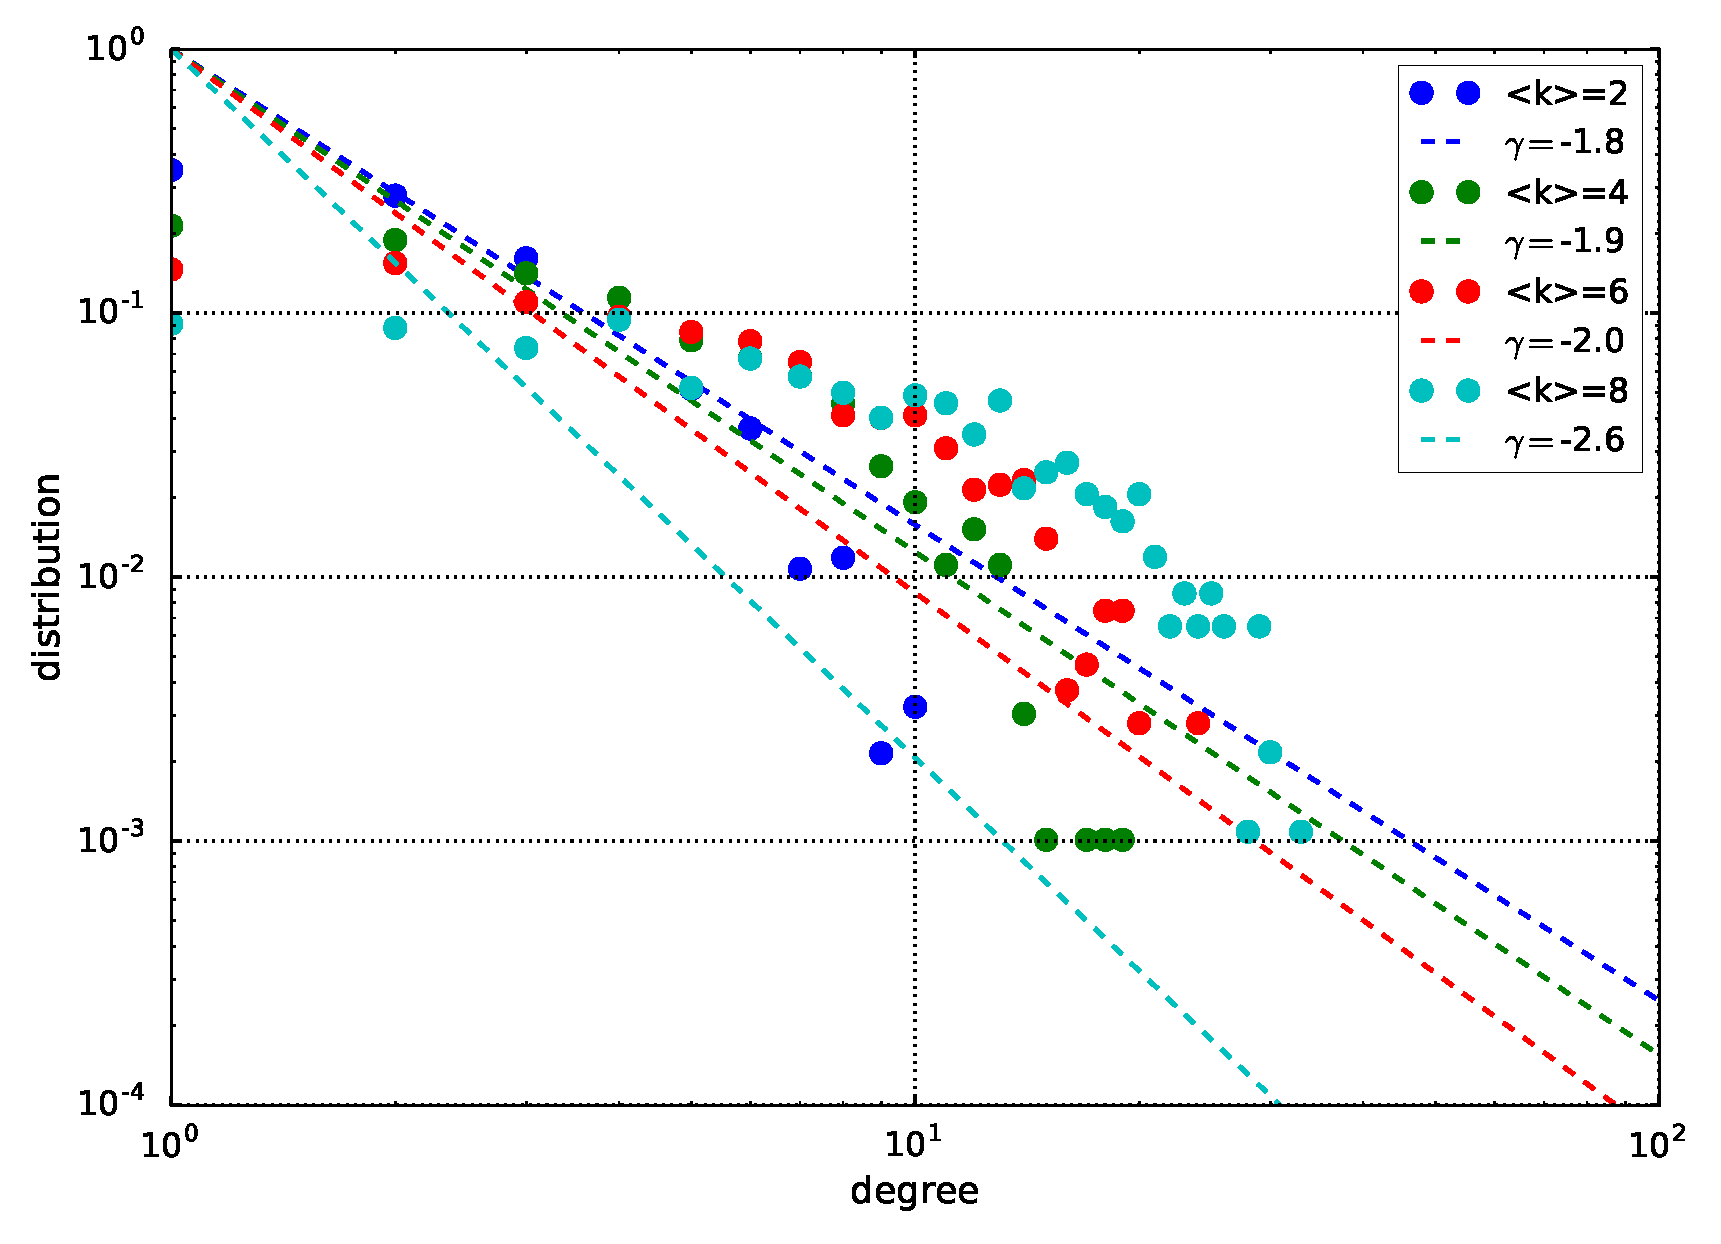
\includegraphics[width=10cm]{powerlaw_degree_dist.eps}
  \caption{Degree distribution of power-law networks of $<k>=2,4,6,8$.
  The fitting curves are depicted by dotted lines.}
  \label{fig_degree}
\end{figure}


\label{centrality,option, corr}
In some contexts, an accurate mathematical
definition for a critical node, particularly for highly complex systems such as the
brain [7], may not yet exist.

As mentioned above, centrality metrics quantify vertex importance in a network based on varying mechanisms.
Here we first review the representative centrality metrics widely used.
\begin{itemize}

\item Degree

Degree is the simplest and the most straightforward metic to measure the importance
of certain individuals, that is, to count the number of vertices who have connected with it.
The presence of few highly connected hubs is the most prominent feature in terms of heterogeneity.
The vertices with the highest degree in the network usually are referred as hubs who
can influence more nodes effectively due to having the greatest number of neighbors.
Degree has been reported indeed play a crucial role in evolutionary games as well as in epidemic and propagation field.
For instance, players with a high degree possess evolutionary advantage due to the larger
number of games they play.
Therefore in the present work, degree is seen as a fundamental metric in PD game.

\item Coreness

Recently, Kitsaket al. \cite{KitsakGallos-17826} argued that the location of a node is
more significant than the number of its linked neighbours, and
they suggested that coreness is a better indicator of a vertex’s
influence on spreading dynamics than degree.
For example, if a hub exists at the end of a branch
at the periphery of a network, it will have a minimal impact
in the spreading process through the core of the network,
whereas a less connected person who is strategically placed in
the core of the network will have a significant effect that leads
to dissemination through a large fraction of the population.
The coreness of a vertex is measured by k-core decomposition \cite{DorogovtsevGoltsev-18309} ,
and a larger coreness value indicates that the vertex is more centrally located in
the network, which implies the topological position of individuals in population perhaps affects evolutionary outcome.

\item H-index

The Hirsch index (also called the H-index)\cite{Hirsch-18310} was originally used
to measure the citation impact of a scholar or a journal \cite{BraunGlänzel-18314}.
For a scholar or journal, the H-index is defined as the maximum value such
that there exists at least h papers, each with citation count.
Recently, Lü, L., et al.\cite{LüZhou-18192} discovered that degree, H-index and coreness are the initial, intermediate and steady states of the sequences, respectively;
and the H-index is a good tradeoff that in many cases can better quantify vertex influence than either degree or coreness.

\item Betweenness
Betweenness \cite{Anthonisse-18331} is one of the most popular geodesic-path-based ranking measures,
which is defined as the fraction of shortest paths between all node pairs that
pass through the node of interest.
L. Freeman \cite{Freeman-18315} has introduced the expression below to compute this centrality,

\item Closeness
Assigns scores to each vertex based on the mean distance to each other vertex.
The closeness \cite{KoschützkiLehmann-18332} of a node i is the average hopcount
of the shortest paths from nodei to all other nodes. It
measures how close a node is to all the others. The most
commonly used definition is the reciprocal of the total
hopcount

Thus, the more central a node is the lower its total distance from all other nodes.

\item Clustering

Clustering Coefficient(CC) was proposed by Duncan J. Watts and Steven Strogatz \cite{WattsStrogatz-18333} in order to determine whether a graph is a small-world network.
For a vertex i, the local clustering coefficient C is the fraction of actual links within its neighborhood to the number of potential links that could possibly exist among them.
In a different context the clustering coefficient characterizes the proportion between the number of observed triangles to all possible triangles as link transitivity in one network, quantifying how close its neighbors are to being a clique (complete graph).
In many cases the presence of clustering structure in the network seems to be the crucial feature responsible for favoring cooperators or defectors\cite{SantosPacheco-18280,Gracia-LázaroCuesta-18325,HuangZheng-18221}.
In the context of evolutionary dynamic, it is reasonable to quantify the influence of a vertex through its clustering coefficient.
Note that CC takes smaller values for more central nodes, in opposite to the other centrality measures.

\item Eigenvector

Besides aforementioned metrics, we also consider another frequently used metric eigenvector centrality,
for a vertex which is defined as the fraction of time that a random walk(er) will spend at that vertex
over an infinite time horizon.
Formally, it is defined by the eigenvector associated to the largest eigenvalue
of the adjacency matrix A of network.
Its variant, Google's PageRank based on the concept that connections to high-scoring sites contribute
more to the score of the site in question than equal connections to low-scoring sites, is more well-known.

\end{itemize}


In order to explorer for this study the influences on the evolutionary outcome
caused by individual importance, we systematically analyzed the properties of aforementioned
centralities, including the distribution of centrality score and correlation.
Although the correlations between centrality metrics have been studied\cite{LiLi-18181,šikićLančić-17843},
the ranked sequence of vertices heavily depends on the dynamical regime and the topological features of network.
It is necessary to investigate the correlation between any two centrality metrics on
the networks used in the present study.
As detailed in Fig.\ref{fig corr centrality k=2} and \ref{fig corr centrality k=8}, we computed the Pearson correlation coefficients
between any two centrality metrics.

\begin{figure}
  \centering
  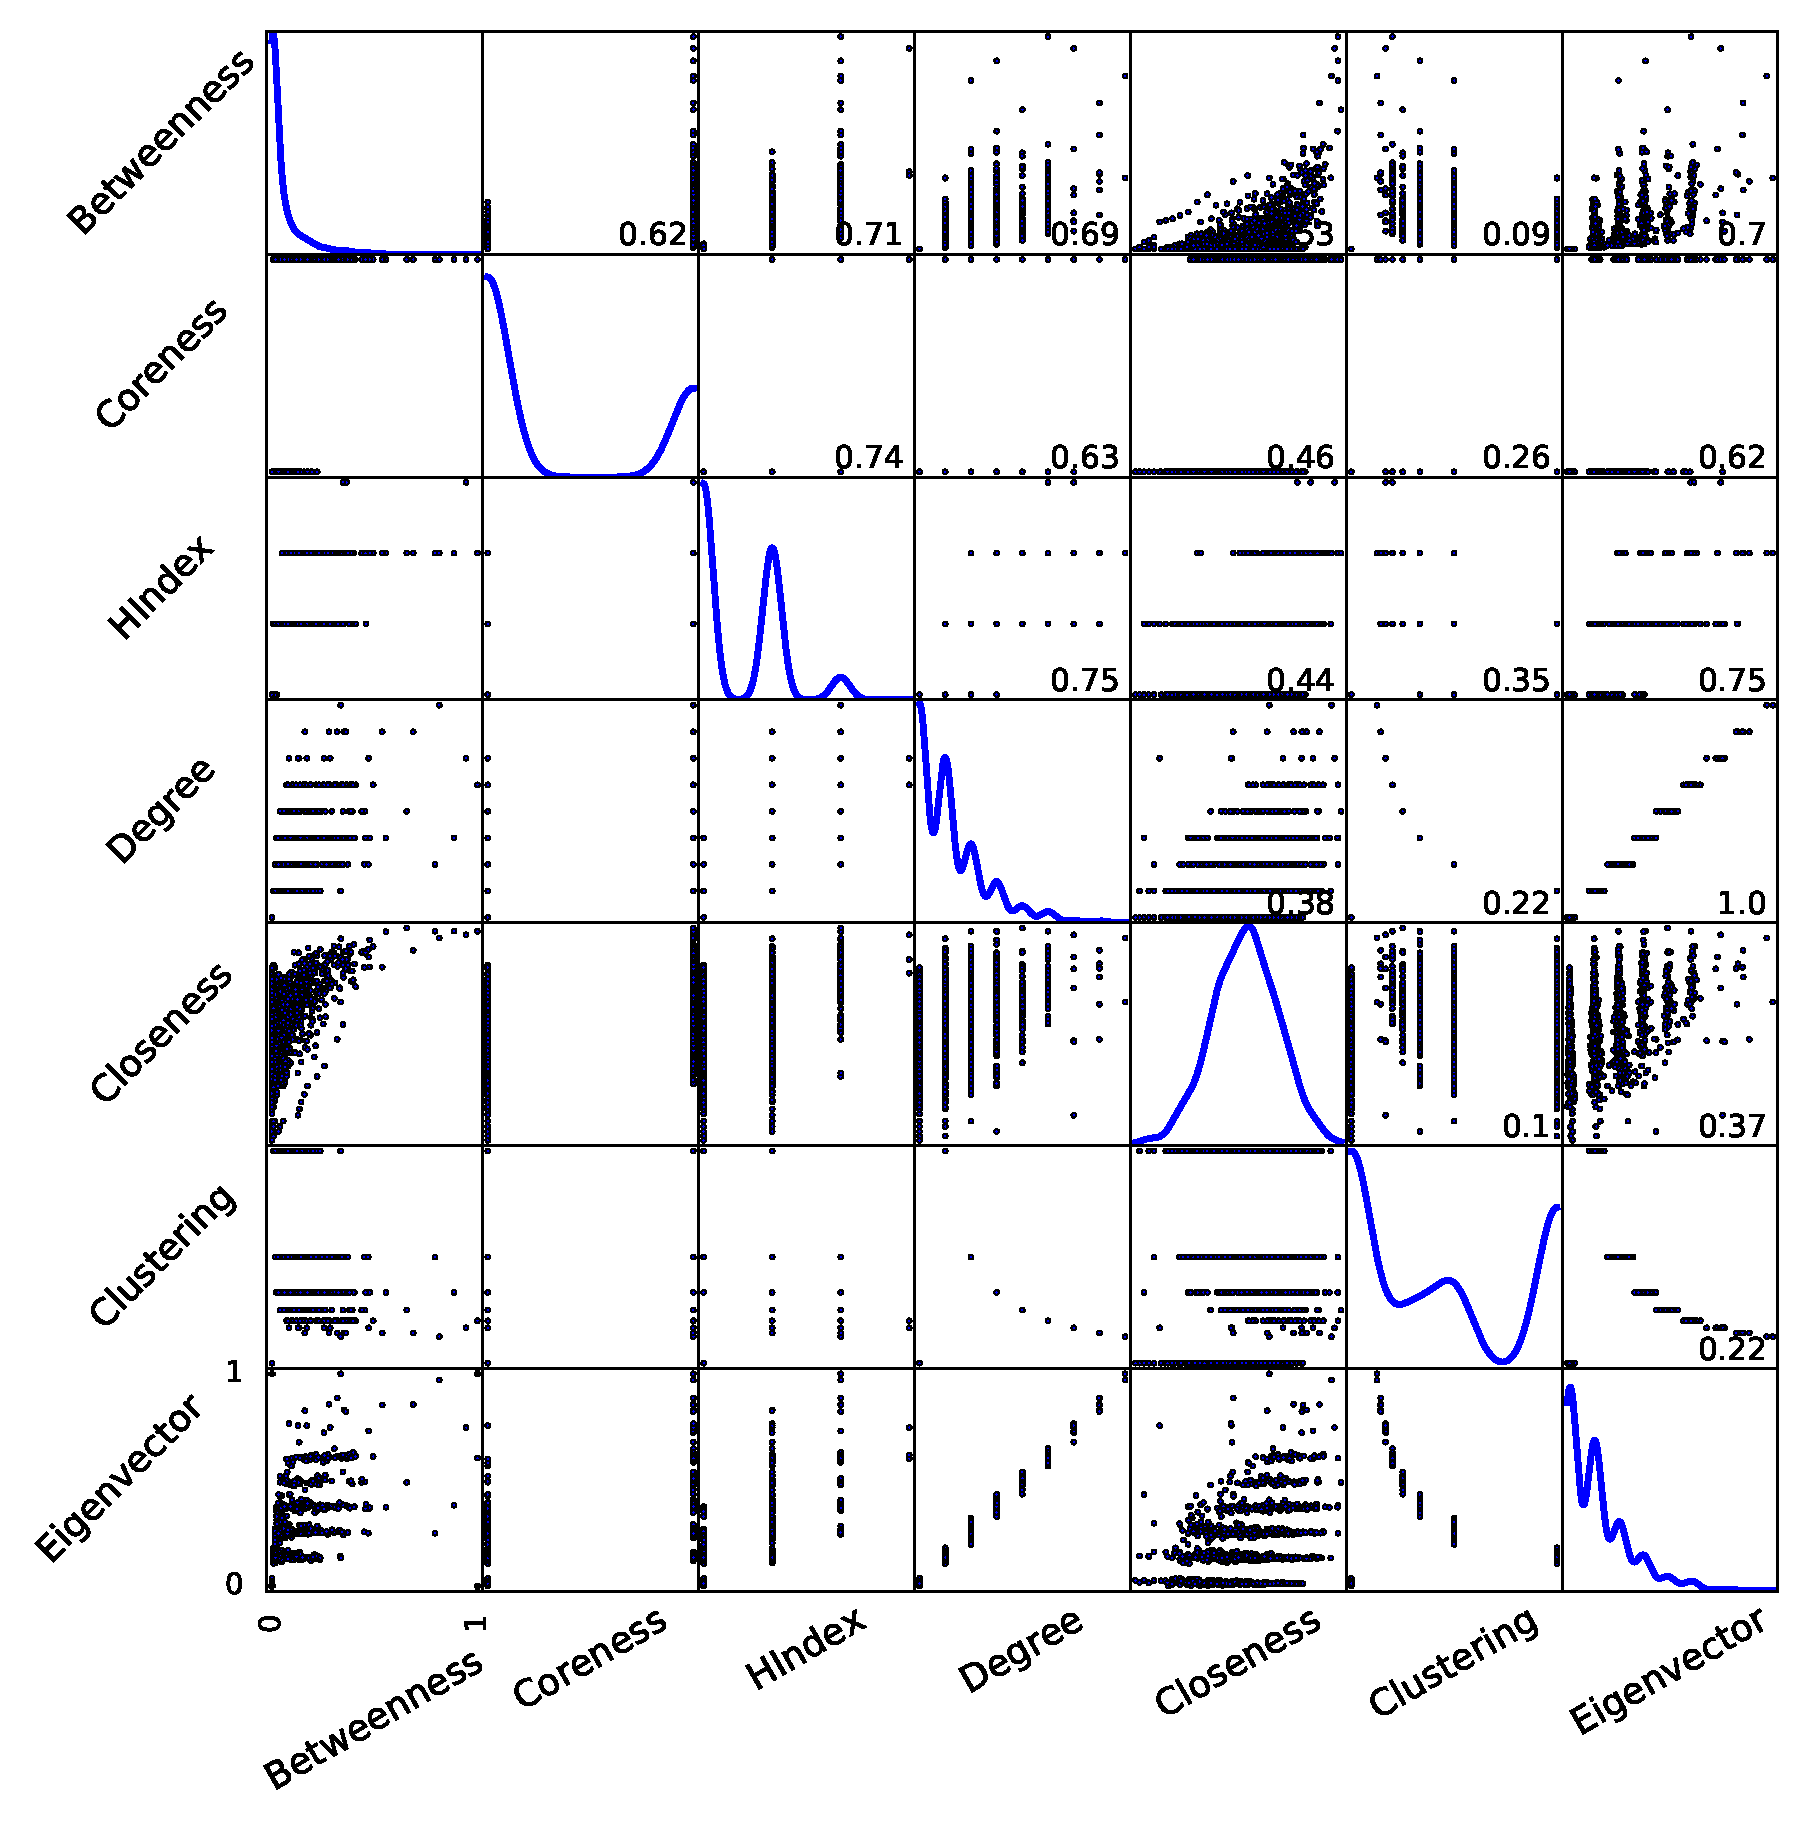
\includegraphics[width=16cm]{Powerlaw_k2_centrality_correlation.eps}
  \caption{Correlation matrix and distributions of centralities considered in this study on network of $<k>=2$.
  The diagonal insets depict density estimation of centralities.
  The Pearson Correlation Coefficients are shown on upper triangular insets.
  Note that the centrality Eigenvector and Degree indicates a perfect positive correlation.
  It also should be noted that centrality Clustering is negatively correlated with all the other centralities.
    }
  \label{fig corr centrality k=2}
\end{figure}

\begin{figure}
  \centering
  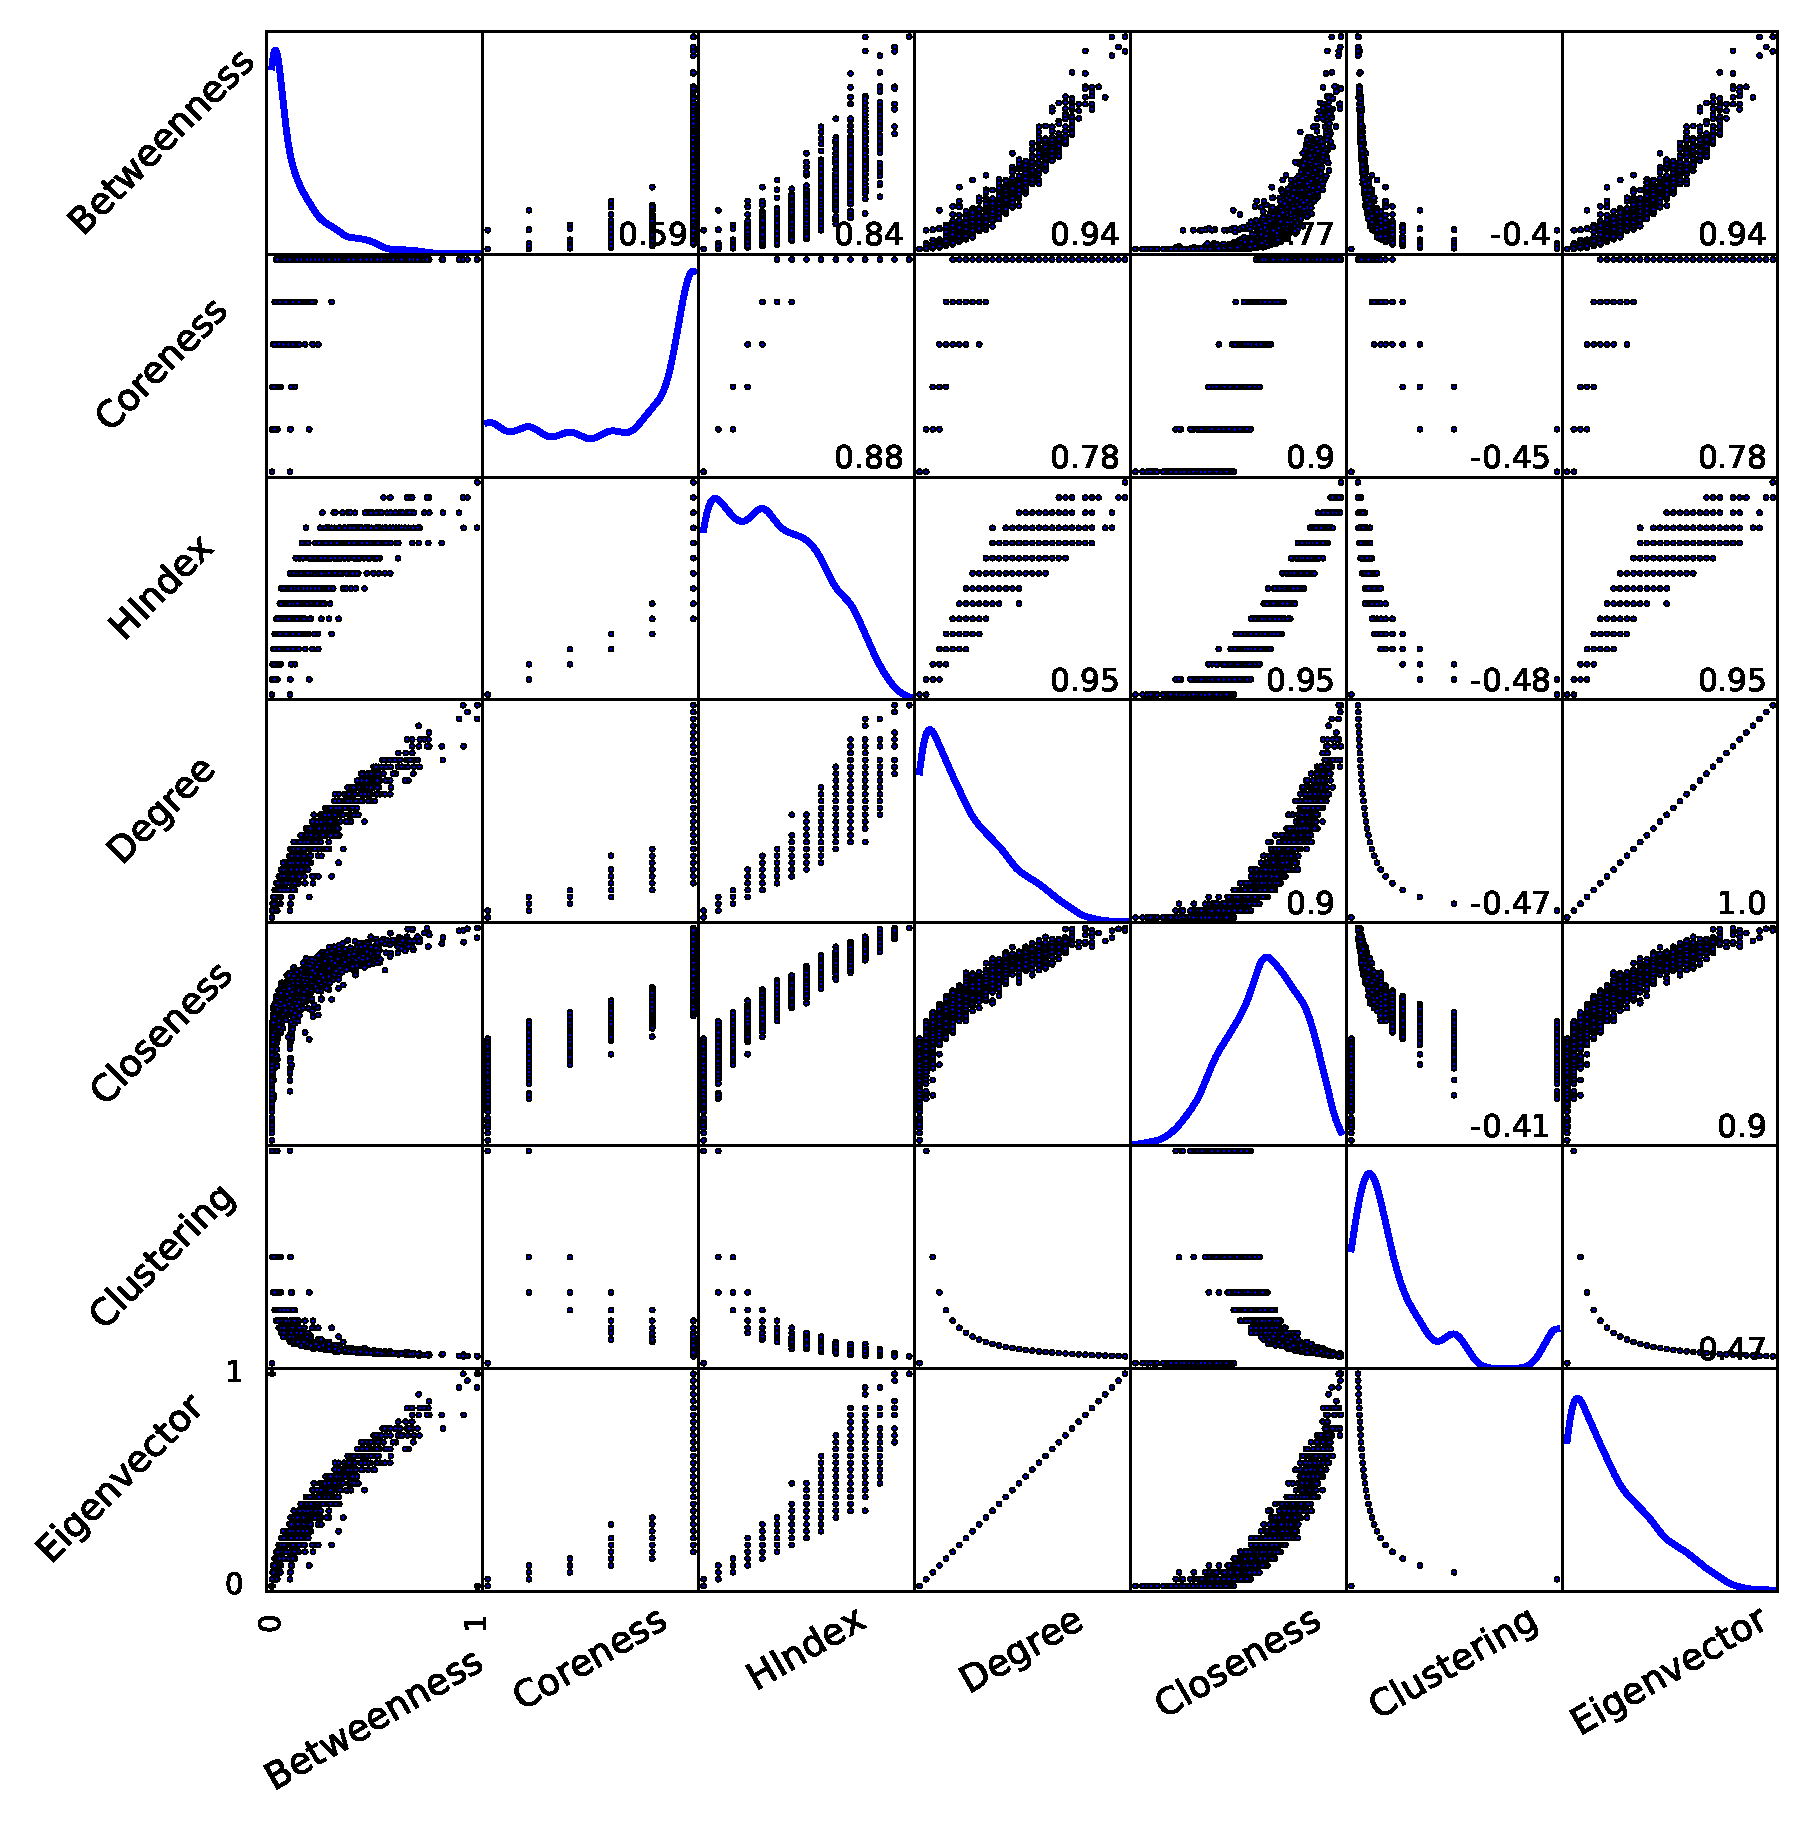
\includegraphics[width=16cm]{Powerlaw_k8_centrality_correlation.eps}
  \caption{Correlation matrix and distributions of centralities considered in this study on network of $<k>=8$..
  }
  \label{fig corr centrality k=8}
\end{figure}

\label{game model}
The evolutionary dynamic is defined as follow.
Two players(individuals) interact with each other through strategies of Cooperation(C) and
Defection(D).
They both get a reward $R$ for mutual cooperation and a punishment $P$ for mutual defection.
If one player cooperates while the other defects, their game payoffs are $S$
(sucker's payoff) and $T$ (temptation), respectively.
Strategists accumulate their payoffs through playing with their own neighbors and the payoff
to a player is in terms of the effect on its fitness.
In the PD game, the ordering of the four payoffs is $T > R > P > S$ , which immediately follows
that the optimum choice for both players is defection regardless of opponent's strategy.
But $2R > T+S$ indicates that mutual cooperation will get higher cumulative income.
Thus, there is a dilemma.
In homogeneous and infinite populations, the individual's selfish and non-cooperative behavior
with short-term benefit will prevail under replicate dynamics  without any specific mechanism.
Obviously this is an unfavorable scenario in the perspective of social progress.
\label{sovle dilemma}Over the past few decades,therefore researchers have proposed various
approaches or mechanisms to solve this dilemma.
Different from traditional practice, here we set $R=2$ and $P=1$ and
correspondingly $0\leq S \leq1$ and $2\leq S \leq3$.
The studied region in the T-S plane we employed was sampled in steps of 0.1,
thus encompassing $11 \times 11=121$ parameter combinations.


We simulate the evolutionary process with synchronous update procedure comprising
discrete elementary steps(game round) where the whole population play simultaneously.
Initially, a portion of individuals  $rho_c (0)$ randomly chosen are assigned cooperation strategy and others defection strategy.
Each round consists of two basic stages.
First, all the individuals in the population play the game once with all their neighbors and obtain
corresponding payoffs according to payoff matrix.
Second, they all update their strategy at once and their payoff is reset to zero before the next
game round.
With strategy updating, we adopted \textit{Fermi rule}\cite{SzabóTőke-18257}.
Player $x$ with strategy $s_x$ imitates the strategy $s_y$ of another player $y$,
chosen randomly from $x’s$ neighborhood, iff $y’s$ strategy has yielded higher payoff,
otherwise player $x$ maintains its original strategy.
Player $x$ takes over the strategy $s_y$  with a probability determined by
the Fermi function

\begin{equation}
\mathcal{P}(s_y^t\rightarrow s_x^{t+1})=\frac{1}{1+e^{-[(P_y^t-P_x^t)]/k}}
\end{equation}
where $k=0.1$ quantifies the uncertainty related to the strategy changing process.
The selected value of $k$ is a traditional and frequently employed choice that does
not qualitatively affect the evolutionary outcomes, as shown in many preceding
works and reviewed comprehensively in \cite{szabo2007evolutionary,wang2014degree}.
In our works, above setups including random initialization of strategy, imitator update rule and parameters
related to PD game xx standard imitator dynamics.

we have found that, for population sizes $N=2000$, times well over 3000 steps
warrants a correct convergence and steady outcome, in agreement with many other works in field, like for example xx.
If the population did not reach full cooperation or defection,
an average of the cooperation density during the last tenth of the evolution was used to obtain
the asymptotic cooperation density.
Moreover, in order to assure suitable accuracy and avoid the stochastic effect all the final results are obtained
via averaging 100 independent runs for each set of parameters.


%%%%%%%%%%%%%%%%%%%%%%%%%%%%%%%%%%%%%%%%%%%%%%%%%%%%%%%%%%%%%%%%%%%
\section{ Results and discussion}

The presentation of the results begins with the standard imitator dynamics
on a series of xx population(see Section xx) which would be seen as benchmark for the following further results.
Fig.\ref{fig power law benchmark} illustrates the impact of average degree $<k>$ and initial proportion of cooperators
 $rho_{c}(0)$ on the outcome of the T-S space panel.
In the first place, it is clearly evidenced that heterogeneity boosts cooperation as verified in a lot of works xx.
Although there are arguments in experiments on this point as for example Carlos Gracia-Lázaro, etl argue that heterogeneous networks do not promote cooperation when humans play a Prisoner’s Dilemma
\cite{Gracia-LázaroFerrer-18206}
, we can confirm this conclusion under the present conditions.
Second, the stable cooperation level depends on the initial condition, which was underestimated in previous works.
The area of full cooperation in the T-S panel is extended With the increase of $rho_{c}(0)$.
And finally, it is suggested that with the average degree increases the networks approximates more and more closely
to the well-mixed structure, which has been proved to be inhibitor toward cooperators.
Consequently,the populations of larger <k> would lead to the lower cooperation level.
However, it can be observed that the influence of <K> is not monotonous toward cooperation level,
<k>=2 being the exception from <k>=4,6,8.
Therefore, we further inspect the conditions of smaller resolution of <k> and the result is given
 in Fig.\ref{fig power law benchmark smallk}.
we observe from Fig.\ref{fig power law benchmark} and Fig.\ref{fig power law benchmark smallk}
that irrespective of  the mean $rho_{c}(\infty)$ on T-S space reaches the maximum when <k=2.7> then declines
In other words, the cooperation level does not monotonously depend on the average degree of underlying network.
This implies the connection density has critical impact on cooperation level even xx.



\begin{figure}[htbp]
\centering
\includegraphics[width=12cm]{powerlaw_random_init_TSPanel.eps}

\caption{Asymptotic density of cooperators $\rho_C$ on the T-S parameter plane.}
\label{fig power law benchmark}
\end{figure}

\begin{figure}[htbp]
\centering
\includegraphics[width=12cm]{powerlaw_smallk_random_init_TSPanel.eps}

\caption{Asymptotic density of cooperators $\rho_C$ on the T-S parameter plane.
The initial densities of cooperators are $\rho_{C}(0)=0.1,0.3,0.5$(columns from left to right).
The average degree of network covers  $<k>$=2(a,b,c),4(d,e,f),6(g,h,i),8(j,k,l).}
\label{fig power law benchmark smallk}
\end{figure}

%%% top rank as cooperator

\begin{figure}[htbp]
\centering
\includegraphics[width=12cm]{PowlawK2topRank.png}

\caption{Asymptotic density of cooperators $\rho_C$ on the T-S parameter plane.

}
\label{k2}
\end{figure}





\section{Conclusion}
it turned out that the rate of cooperation is affected by the strategy set, the evolutionary rules, the payoffs, and the structure of connectivity.
For such a high degree of freedom the analysis cannot be complete.
In many cases investigations are carried out for a payoff matrix with a limited number of variable parameters.
Even for the same factor mentioned above, there are still arguments,
i.e. the effect of population structure on cooperation level.

it turned out that the cooperation level is affected by the strategy set,
the evolutionary rules, the payoffs, and the structure of connectivity.
For such a high degree of freedom the analysis cannot be complete.

As network science evolves\cite{albert2002statistical} , the focus of evolutionary theory is shifting
from macroscopic to reveal the role played by such microscopic factors as individuals in the structured
population.

Although recent large-scale human experiments indicate that spatial reciprocity
 may be compromised or fail altogether, there is still ample interest in understanding
 how and why networks influence the evolution of cooperation.

this conclusion is strengthened and quantitatively corroborated.

we would like to point out that all our results remain unchanged both for larger and smaller population size.
The present results demonstrate that, in more realistic, heterogeneous populations, the sustainability of cooperation is simpler to achieve than in homogeneous populations, a result that is valid irrespective of the dilemma adopted as a metaphor of cooperation.

despite the vitures of this paper, we consider that two important shortcomings render it a preliminary and inconclusive attempt: (1)xx; and (2) xx.

We have found an unquestionable
dependence of the evolutionary outcome on the update
rule, which has in turn consequences on the robustness
of the spatial effects and on the in
uence of the synchronicity of the updating.

generalize know results to wider sets of games and spatial structure of population.
allow to integrate apparently contradictory results in the literature.
have reached additional conclusions.

our simulations and outcomes evidence that there is no absolutely best metrics identifying influential
cooperators independent of the environment.

In particular, we will focus our attention in one topological feature: centrality.
Since the most central nodes can diffuse their influence to the whole network faster than
the rest of nodes. A natural inference is expected that such agents are the most influential spreaders.

Centrality.The meaning for evolutionary game
1. Opportunity of connecting to more individuals.
2. Able to obtain more information.
3. Potential payoffs for long term of cooperation.
4. Centrality is relatively easier to obtain or evaluate compared with payoffs

\appendix


%% References
%%
%% Following citation commands can be used in the body text:
%% Usage of \cite is as follows:
%%   \cite{key}         ==>>  [#]
%%   \cite[chap. 2]{key} ==>> [#, chap. 2]
%%

%% References with bibTeX database:

\bibliographystyle{elsarticle-num}
% \bibliographystyle{elsarticle-harv}
% \bibliographystyle{elsarticle-num-names}
% \bibliographystyle{model1a-num-names}
% \bibliographystyle{model1b-num-names}
% \bibliographystyle{model1c-num-names}
% \bibliographystyle{model1-num-names}
% \bibliographystyle{model2-names}
% \bibliographystyle{model3a-num-names}
% \bibliographystyle{model3-num-names}
% \bibliographystyle{model4-names}
% \bibliographystyle{model5-names}
% \bibliographystyle{model6-num-names}

\bibliography{references}


\end{document}

%%
%% End of file `elsarticle-template-num.tex'.
